\chapter{Description du travail réalisé}
\setlength{\parskip}{2.5ex plus .4ex minus .4ex}

\section{Architecture}
\subsection{Plugin global}
Afin de répondre au besoin, il a été décidé de développer un plugin global dans un paquet appelé vle.ibm.\\
Un plugin global est une extension de logiciel permettant de mettre à disposition de l'utilisateur des fonctionnalités additionnelles. Cette extension se différencie d'un plugin classique par le fait qu'il ait accès au logiciel entier, à toutes ses informations, fonctionnalités...\\
Cependant, faire un plugin global a obligé quelques modifications des fichiers sources du logiciel. En effet, certaines informations étaient privées et il était nécessaire d'y accéder. Ce qui m'a obligé à bien comprendre la structure du logiciel grâce aux éléments que j'avais en main, fichiers sources et documentation, afin d'y insérer les bonnes méthodes correspondantes à mes besoins.

\subsection{Arguments}
Les raisons de cette décision sont variées. L'extension a besoin d'accéder à toutes les classes d'individu déjà créées par l'utilisateur précédemment dans le Vpz et qu'il puisse en créer de nouvelles depuis le plugin, afin que le clonage d'individus soit faisable. Le plugin a aussi besoin d'avoir accès au Vpz entier (conditions expérimentales, ports,...) et donc de VLE, car il intéragit avec ce dernier lors de la simulation.\\
De plus, une interface graphique du plugin devait être développée afin d'en faciliter l'utilisation, c'est pourquoi l'accès à GVLE\footnote{GUI pour VLE} était également indispensable.\\

Le plugin développé permet le lancement du plugin Forrester afin de créer les classes d'individu et est en lien avec un proxy permettant la communication entre le langage de script proposé à l'utilisateur et le controleur.\\

VLE est un logiciel fonctionnant grâce à des paquets, ils peuvent contenir un projet, un Vpz, une extension... Par exemple, le plugin Forrester fait parti du paquet vle.forrester, le plugin IBM est dans le paquet vle.ibm.\\

\noindent\begin{minipage}{\linewidth}% to keep image and caption on one page
\makebox[\linewidth]{%        to center the image
  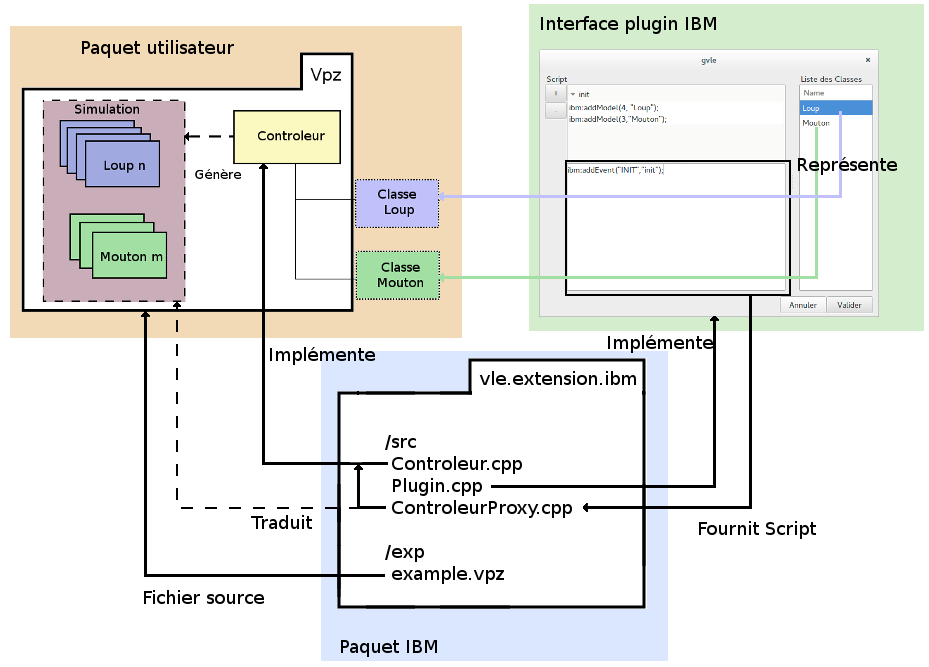
\includegraphics [width=150mm]{images/architecture.png}}
\captionof{figure}{Architecture du système}%\label{visina8}%      only if needed
\end{minipage}

Ici, deux paquets, vle.ibm en bleu et le paquet de projet de l'utilisateur en jaune. Le plugin IBM offre l'interface d'ibm où l'utilisateur décrit ses besoins puis il met en place le controleur grâce à ces informations. Le Controleur peut alors générer les individus lors de la simulation.

\section{Controleur}
L'élément principal du système IBM est le controleur, il a pour but de gérer tous les évènements qui voyagent dans le système en les faisant passer par lui. Il hérite de nombreuses classes ce qui lui permet d'avoir les capacités d'une dynamique, d'un exécutive et d'un GenericAgent.\\
\noindent\begin{minipage}{\linewidth}% to keep image and caption on one page
\makebox[\linewidth]{%        to center the image
  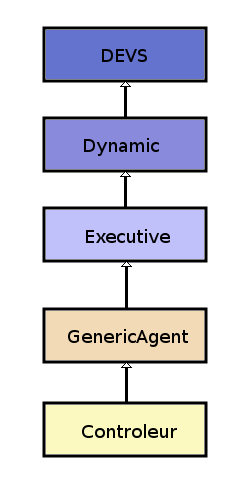
\includegraphics [width=60mm]{images/heritageControleur.png}}
\captionof{figure}{Graphe d'héritage du controleur}%\label{visina8}%      only if needed
\end{minipage}

Il se crée automatiquement à la première ouverture du plugin IBM. Ces capacités sont multiples grâce à la hiérarchie d'héritage dont il est formé.
\subsection{Une dynamique}
Il possède la capacité d'une dynamique DEVS, recevoir des évènements par ses ports d'entrée, envoyer des évènements par ses ports de sortie, exécuter un programme interne à chaque pas de temps (transition interne), gérer les évènements externes (transition externe). Voici un résumé de sa dynamique. \\
\noindent\begin{minipage}{\linewidth}% to keep image and caption on one page
\makebox[\linewidth]{%        to center the image
  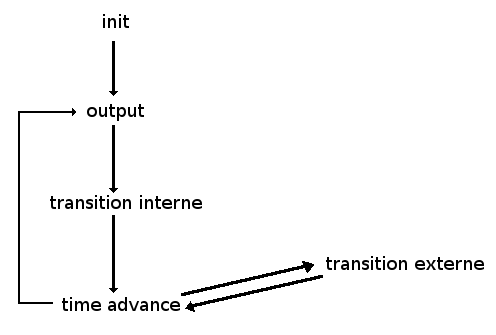
\includegraphics [width=100mm]{images/dynamiqueControleur.png}}
\captionof{figure}{Dynamique du controleur}%\label{visina8}%      only if needed
\end{minipage}

Le controleur s'initialise dans init, puis exécute en boucle output, transition interne et time advance. \\
Output envoie les évènements par les ports de sortie, transition interne exécute les tâches régulières du controleur à chaque pas de temps t rendu par time advance.\\
La transition externe quant à elle s'exécute lors de la réception d'évènements, les traite puis la dynamique continue son cycle depuis time advance.

\subsection{Un executive}
Héritant d'``Exécutive'', le controleur a le pouvoir de créer des modèles mais aussi de les détruire et les modifier.\\
En effet, afin de créer des clones et les manipuler suivant les souhaits de l'utilisateur, le Controleur a besoin de ces capacités.\\
Pour cela, un petit langage sera mis à la disposition de l'utilisateur afin qu'il puisse programmer les agissement du Controleur durant la simulation. \\
Ce petit programme est une chaine de caractère exécutée par le Controleur au bon moment grâce à sa dynamique afin de respecter les dates d'agissement souhaitées par l'utilisateur.

\subsection{Le scheduler}
Le Controleur hérite également de GenericAgent, ce qui lui donne accès à une sorte de calendrier. Il peut ainsi créer des évènements, les enmagasiner et exécuter les scripts envoyés par ces évènements à la bonne date.

\section{GUI}
Une interface simple a été développée pour l'utilisateur. Trois champs principaux en vert, rouge et les nuances de bleu ci-dessous.\\
La colonne de droite en vert qui liste toutes les classes d'individu présentes dans le Vpz ouvert. En survolant le nom d'une classe une infobulle s'ouvre pour afficher la liste des paramètres et compartiments de la classe en question, ce qui permet à l'utilisateur de programmer plus facilement. Il a directement accès à toutes les variables potentiellement modifiables au cours de la simulation.\\
Par un clique-droit sur la colonne des classes, un menu déroulant s'affiche où l'utilisateur peut décider de créer une nouvelle classe, modifier la classe sélectionnée ou la supprimer.\\
En rouge la zone de texte permettant l'écriture du script lua qui peut être des appels à évènements, des fonctions et/ou des initialisations de variables. Ce script n'est appelé qu'une fois en début de simulation.\\
En bleu, les évènements, on peut en ajouter grâce au bouton ``+'' sur le coté gauche ou en supprimer grâce au bonton ``-''. Le nom de l'évènement est en évidence après chaque flèche et le script correspondant est juste en dessous.\\

Ici l'exemple du tp Modelmaker sur le remplissage et vidange des compartiments.
Deux évènements, ``exec'' et ``init'', ``init'' est appelé lors de l'initialisation et le script de l'évènement ``exec'' tous les 0.1 à partir de la date 0.01.

\noindent\begin{minipage}{\linewidth}% to keep image and caption on one page
\makebox[\linewidth]{%        to center the image
  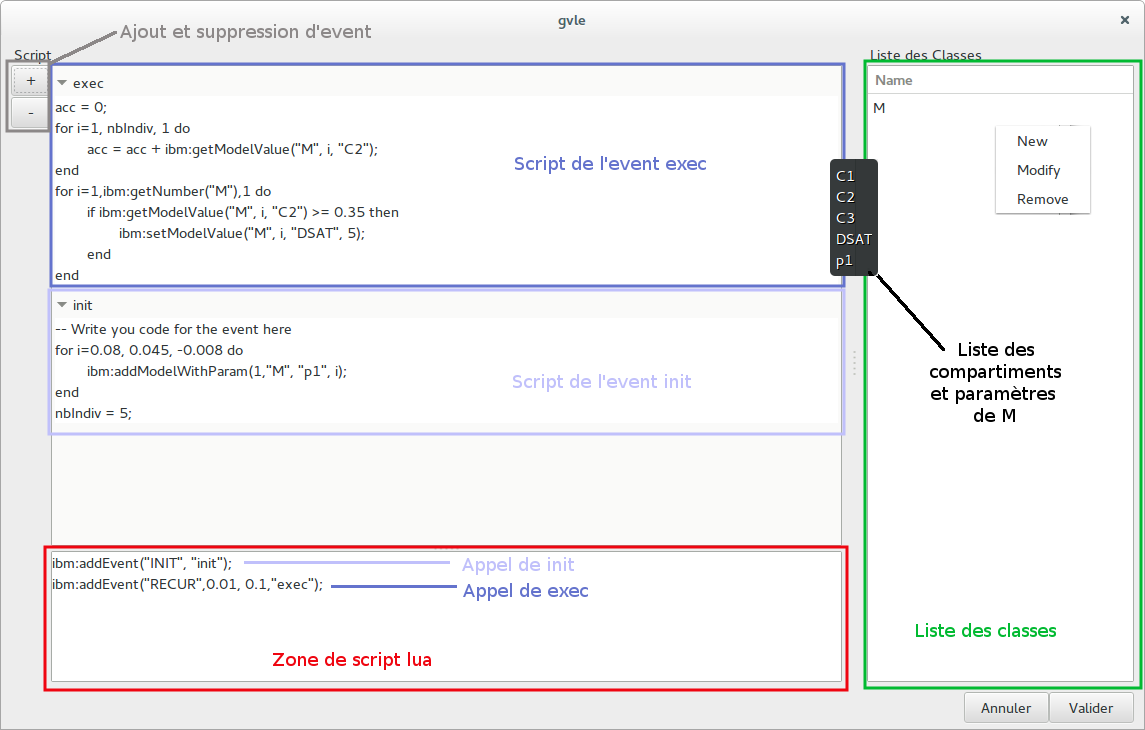
\includegraphics [width=150mm]{images/exemplePlugin.png}}
\captionof{figure}{Interface graphique du plugin IBM}%\label{visina8}%      only if needed
\end{minipage}

\section{Lua \& addons}
Lua est un langage de script libre créé en 1993. Il a été conçu de manière à pouvoir être embarqué et augmenter les possibilités du système hôte.\\
Dans notre cas, il sert d'interprète entre ce que l'utilisateur souhaite faire et le controleur. Ainsi, on peut profiter de tout le langage lua, plus quelques fonctionnalitées que j'ai développées qui permettent certaines actions précises sur les individus.\\
\subsection{Mise en oeuvre}
Un script lua peut très facilement être exécuté depuis un programme C++. \\
On retrouvera les principales structures for, while, if, l'utilisation de variable... que l'utilisateur pourra se servir dans son script.\\
Mais ce langage ne permet pas à l'utilisateur d'effectuer des actions sur les individus. C'est pourquoi, des extensions à ce langage ont été développées et sont exécutées grâce à l'intermédiare d'un proxy.\\
\\
Dans l'exemple ci-dessous, le Controleur récupère le script lua puis l'exécute. Comme addModel n'existe pas dans le langage lua, le proxy comblera cette anomalie en appelant la fonction du Controleur associée à addModel à chaque fois qu'elle sera appelé. Dans ce cas, trois fois.\\

\noindent\begin{minipage}{\linewidth}% to keep image and caption on one page
\makebox[\linewidth]{%        to center the image
  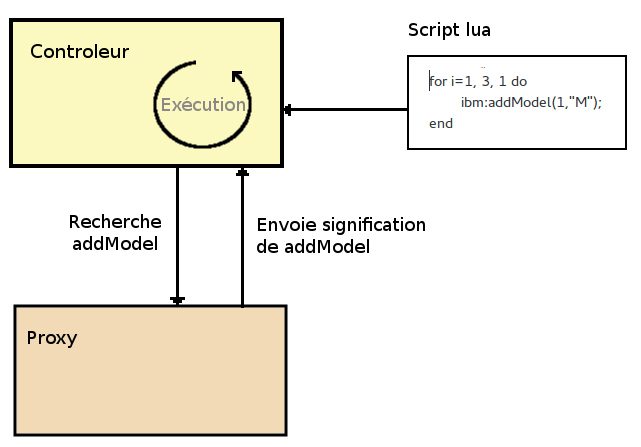
\includegraphics [width=150mm]{images/proxyLua.png}}
\captionof{figure}{Exécution d'un script lua depuis le controleur}%\label{visina8}%      only if needed
\end{minipage}

\subsection{Les extensions}
Chaque extension du langage lua ont comme préfixe ``ibm\string:''. Elles permettent d'avoir des effets sur les modèles, d'obtenir des informations ou lancer des évènements.\\
Voici la liste des extensions développées qui ont des effets sur les individus :
\begin{itemize}[label=\textbullet,font=\large]
	\item addModel(n,``M'')\\
	Ajoute n models de type ``M''.
	\item delModel(``ModelName'')\\
	Supprime le modèle dont le nom est ``ModelName''.
	\item addModelWithParam(n, ``Class'', ``Param1'', value1, ``Param2'', value2, ...)\\
	Ajoute n model de type ``Class'' en modifiant les paramètres de telle manière à ce que Param1 = value1 et Param2 = value2. Le nombre de paramètre à modifier est indéfini.
	\item setModelValue(``class'', i, ``varName'', varValue)\\
	Modifie la valeur de ``varName'' par ``varValue'' du i\up{ème} modèle de la classe ``class''.
	\item setModelValue(``modelName'', ``varName'', varValue)\\
	Modifie la valeur de ``varName'' par ``varValue'' du modèle nommé ``modelName''.
\end{itemize}
Les extensions qui permettent d'avoir des informations sur les individus.
\begin{itemize}[label=\textbullet,font=\large]
	\item getModelValue(``modelName'', ``varName'')\\
	Renvoie la valeur de la variable ``varName'' du modèle dont le nom est ``modelName''.
	\item getModelValue(``class'', i, ``varName'')\\
	Renvoie la valeur de la variable ``varName'' du i\up{ème} modèle de la classe ``class''.
	\item getModelName(``class'',i)\\
	Renvoie le nom du i\up{ème} modèle de la classe ``class''.
	\item getNumber(``class'')\\
	Renvoie le nombre d'individu de la classe ``class''.
	\item getTime()\\
	Renvoie la date actuelle durant la simulation.
	\item getParam(``param'')
	Renvoie la valeur du paramètre ``param'' présent dans les conditions expérimentales du controleur.
\end{itemize}

Dans toutes ces extensions, il est possible de remplacer la valeur des quantités, double ou int, par une chaîne de caractère qui correspond à un paramètre des conditions expérimentales du Controleur.\\
Quantité de modèles ajoutés dans addModel, la quantité de modèles et la valeur des paramètres dans addModelWithParam et la valeur de ``varValue'' dans setModelValue.\\

L'extension permettant de lancer des évènements est addEvent. Cette fonction peut être de trois types, ``INIT'', ``SINGLE'' ou ``RECUR'' préciséd en premier paramètre. \\
L'évènement lancé se traduit par l'exécution d'une fonction écrite par l'utilisateur dans le script. Cette fonction est toujours précisée en dernier paramètre de addEvent.\\
``INIT'' permet de lancer un premier script à l'initialisation de la simulation.\\
``SINGLE'' permet de lancer un évènement ponctuel dans la simulation, c'est-à-dire l'exécution d'une fonction lua à un temps déterminé par l'utilisateur. La syntaxe sera addEvent(``SINGLE'', date, ``fonction'').\\
``RECUR'' permet de lancer un évènement qui s'exécutera à une certaine fréquence depuis une date déterminée par l'utilisateur et jusqu'à la fin de la simulation. On aura addEvent(``RECUR'', date, frequence, ``fonction'').\\

Par exemple, ici deux évènements sont implémentés.\\
Initialisation, 5*``nbLoup'' loups sont créés. À chaque tour de boucle ``nbLoup'' loups sont créés avec age=1 puis age=2 ... et age=5.

%\noindent\fbox{\begin{minipage}{1.0\textwidth}
%- -Event init\\
%for i=1,5,1 do\\
%	\textcolor{red}{ibm\string:addModel}(``nbLoup'',``Loup'',``age'',i);\\
%end
%\end{minipage}}

\begin{lstlisting}[frame=single]
--Event init
for i=1,5,1 do
	ibm:addModel("nbLoup","Loup","age",i);
end
\end{lstlisting}

Ici, l'évènement ``dyn'' ajoute 1 à l'age de chaque loup. Ceux qui atteignent 10 sont affichés.
\begin{lstlisting}[frame=single]
--Event dyn
for i=1,ibm:getNumber("Loup"),1 do
	x = ibm:getModelValue("Loup",i,"age")
	ibm:setModelValue("Loup",i,"age",x + 1)
	if ibm:getModelValue("Loup",i,"age") == 10 then
		print(ibm:getName("Loup",i))
	end
end
\end{lstlisting}

Appel des évènements. Tout d'abord ``init'' à l'initialisation puis l'évènement ``dyn'' à partir de la date 4 et tous les 1 jusqu'à le fin de la simulation.

\begin{lstlisting}[frame=single]
ibm:addEvent("INIT","init");
ibm:addEvent("RECUR",4,1,"dyn");
\end{lstlisting}

En rouge, toutes les extensions utilisées dans le script.

Une autre fonctionnalité a été implémentée afin de permettre à l'utilisateur d'observer les variables de son choix faisant partie de son script lua.\\
Par exemple, l'utilisateur peut observer la quantité d'individus au cours de la simulation en définissant une variable globale ``var'' dans le  script d'un évènement appelé récursivement qui prendrait pour valeur la somme de tous les individus.\\ Puis l'utilisateur doit déclarer cette variable ``var'' dans les observables du Controleur et lui associer une vue de sortie. Il sera alors possible d'observer la quantité d'individus tout au long de la simulation.
\section{Déroulement du stage}
\subsection{Découverte}
Les premiers jours ont été destinées à l'installation de toutes les parties nécessaires au fonctionnement du logiciel et à la compréhension de ce dernier, à quoi sert-il et comment fonctionne-t-il du point de vue de l'utilisateur.\\
\\
Durant cette phase, j'ai lu la documentation associée à l'utilisation du logiciel afin de comprendre comment était représenté un individu, comment une simulation fonctionnait, l'envoie de messages entre modèles...\\
De plus, j'ai effectué un TP destiné à apprendre à utiliser le plugin Forrester, lancer des simulations et observer les valeurs de certains paramètres.\\
J'ai également réalisé à la main le clonage d'un individu en modifiant un de ses paramètres afin d'avoir une idée plus claire de ce qu'on attendait de moi durant ce stage.
\subsection{Langage de script}
Il était dès le départ évident que l'utilisateur devra programmer une petite partie afin de décrire la vie des individus qu'il aura créé.\\
J'ai tout d'abord commencé à développer les extensions de lua décrites précédemment par l'intermédiaire d'un parser en C++ dans le controleur sans le langage lua. Et seules ces fonctionnalités pouvaient être appelées.\\
Cette méthode était très limitée, c'est pourquoi l'insertion d'un langage existant était nécessaire.\\
Lua, un langage de programmation très simple, se mélange parfaitement au C++ et permet une plus grande liberté à l'utilisateur. Créant un proxy afin de faire l'intermédiaire entre lua et les fonctions C++, l'utilisateur peut profiter de tous les avantages et multiplier ses possibilités.\\
Après la mise en place du proxy, le développement de nouvelles extensions s'est fait sans difficultés.
\subsection{La dynamique}
Après avoir pris connaissance du logiciel et ses fonctionnalités, il m'a fallu comprendre la dynamique de fonctionnement c'est-à-dire la dynamique DEVS. Elle se traduit par l'ordre dans l'exécution des fonctions dans une dynamique, reception d'évènements, envoie d'évènements, transitions interne et externe...\\
A la base, l'utilisateur devait programmer deux scripts, un pour l'initialisation et un autre qui s'exécuterait en continu en transition interne. \\
Cependant, j'ai été confronté à un problème. L'utilisateur ne pouvait pas décider d'exécuter une commande à un moment déterminé au cours de la simulation, par exemple si l'utilisateur souhaite faire naître deux loups à la moitié de la simulation. Pour cela, il devait passer par l'intermédiaire de booléen, ce qui compléxifiait énormément le code et le ralentissait.\\
Afin de résoudre ce problème, j'ai mis en place un Scheduler. Il permet l'ordénation d'évènements par le temps auxquel ils doivent s'exécuter puis l'envoie de ses derniers à la bonne date lors de la simulation.\\
Grâce au Scheduler, l'utilisateur simplifie son code en ne faisant que des fonctions lua puis appelle ses dernières dans l'ordre et la fréquence qu'il souhaite grâce à la commande d'ajout d'évènement addEvent.
\subsection{Bugs \& tests}
Au cours du développement, de nombreux bugs se sont manifestés. Leurs résolutions étaient parfois évidente, mais il pouvait aussi être plus difficil de trouver leurs sources. En effet, ils étaient parfois dû à mon propre code, mais travaillant sur une version de VLE en développement, les bugs pouvaient cependant être dû à l'instabilité de l'application. C'est pourquoi, j'ai effectué des rapports de bug.\\

Afin de repérer les sources d'erreurs plus facilement, j'ai utilisé gdb, mais parfois ce système ne fonctionnait pas car c'était gdb lui-même qui provocait les bugs.\\
D'autres bugs n'étaient visibles que lors de l'analyse des résultats obtenus après simulation. Pour remonter jusqu'aux erreurs, il a fallu songer à des tests, des scripts lua plus simples mais qui pourtant reproduisaient le bug.\\
Après avoir réalisés ces tests, les plus pertinents ont été insérés dans le paquet vle.ibm avec les TP donnés à titre d'exemple des besoins, afin que l'utilisateur en téléchargeant le plugin, puissent avoir des exemples d'implémentations simples.

\subsection{Outils \& organisation}
J'ai développé le plugin vle.ibm par l'intermédiaire de gedit de manière totalement libre grâce au gestionnaire de version GIT et le dépôt Github.\\
Nous avons fait une prémière réunion avec l'équipe-projet Record afin de clarifier ce que je devrais développer en début de stage. Des réunions très régulières avec mon tuteur ont eu lieu dans le but de vérifier mon avancée et envisager les possibilités futures de développement.\\
De plus, j'avais à ma disposition des User Stories qui décrivaient ce que l'utilisateur devait pouvoir réaliser avec le plugin afin de me diriger dans mon développement. Ces User Stories étaient progressives, elles partaient de fonctionnalités simples comme afficher le bouton de démarrage du plugin à la mise en place du Scheduler.\\
Afin de vérifier que toutes les fonctionnalités étaient bien mise en place, j'ai modélisé les systèmes demandés dans les deux TP des besoins, croissance des cellules et vidange des compartiments, mais j'ai aussi réalisé une fiche de cas d'utilisation.\\
Cette fiche, disponible dans le paquet vle.ibm, décrit 21 cas d'utilisation simples permettant à l'utilisateur d'utiliser chacune des extensions que j'ai développées. Chaque cas est détallé afin qu'un utilisateur occasionnel puisse bien comprendre les fonctionnalités du plugin.

\subsection{Planning}
Trois importantes réunions ont eu lieu. Une en début de stage le 27 juin avec l'équipe VLE qui avait pour but de définir la manière d'intégrer les nouvelles fonctionnalités au logiciel GVLE.\\
Une seconde a eu lieu le 9 août par l'intermédiaire de jipsi\footnote{Système de visioconférence} avec les principaux futurs utilisateurs, du plugin IBM afin de faire un état d'avancement.\\
Pour la dernière réunion, le 4 août, ces principaux utilisateurs sont venus sur le site de Toulouse afin que je leur explique le fonctionnement du plugin.

\vspace{-10cm}
\begin{landscape}
%\thispagestyle{empty}
%\thispagestyle{plain}
\setlength{\topmargin}{25pt}
\titlespacing{\subsection}{0cm}{0cm}{0cm}


\noindent\begin{ganttchart}[
hgrid,
vgrid,
inline,
time slot format=stardate
]{2014.167}{2014.215}
\gantttitlecalendar{year, month=name, day} \\
\ganttbar{Compréhension du sujet}{2014.167}{2014.188}
\ganttbar{Developpement fenêtre principale du plugin}{2014.189}{2014.206}
\ganttbar{Mise en place proxy lua}{2014.207}{2014.215}\\
\ganttbar{Lecture documentation}{2014.167}{2014.174}
\ganttmilestone{Réunion d'organisation}{2014.177}
\ganttbar{Prise de connaissance du code source}{2014.180}{2014.200}\\
\ganttbar{Réalisation du TP Forrester}{2014.170}{2014.185}
\ganttbar{Debogage}{2014.202}{2014.215}
\end{ganttchart}

\noindent\begin{ganttchart}[
hgrid,
vgrid,
inline,
time slot format=stardate
]{2014.216}{2014.264}
\gantttitlecalendar{year, month=name, day} \\
\ganttbar{Développement extensions lua}{2014.216}{2014.230}
\ganttbar{Rapport de Stage}{2014.230}{2014.252}
\ganttbar{Congé}{2014.253}{2014.263}\\
\ganttmilestone{Réunion d'avancement}{2014.220}
\ganttbar{Mise en place du Scheduler}{2014.223}{2014.231}
\ganttbar{Modification GUI}{2014.233}{2014.238}
\ganttmilestone{Présentation du plugin}{2014.246}\\
\ganttbar{Tests}{2014.218}{2014.244}\\
\ganttbar{Debogage}{2014.216}{2014.250}
\end{ganttchart}
\end{landscape}

